\subsection{Discretização da pá}

A superfície da pá é amostrada, formando uma grade de tamanho fixo. A técnica
\textit{axis-aligned bounding box (AABB)} é utilizada para obter os
pontos e suas respectivas normais, na superfície da pá. Nesta técnica, a
superfície alvo é inscrita em um bloco, que é uniformemente amostrado. É, então,
realizada uma verificação de colisão entre os pontos amostrados no bloco e a
superfície alvo e, caso haja interseção, o ponto é armazenado junto com sua
normal à superfície. Dessa forma, podemos amostrar a pá e deslocar estes pontos
230 mm em relação à sua normal com a superfície, garantindo a requerimento do
revestimento. A representação dos pontos amostrados e deslocados em relação às
normais da pá estão nas figuras~\ref{fig::amostrapa1} e ~\ref{fig::amostrapa2}. 

\begin{figure}[!ht]
	\centering	
	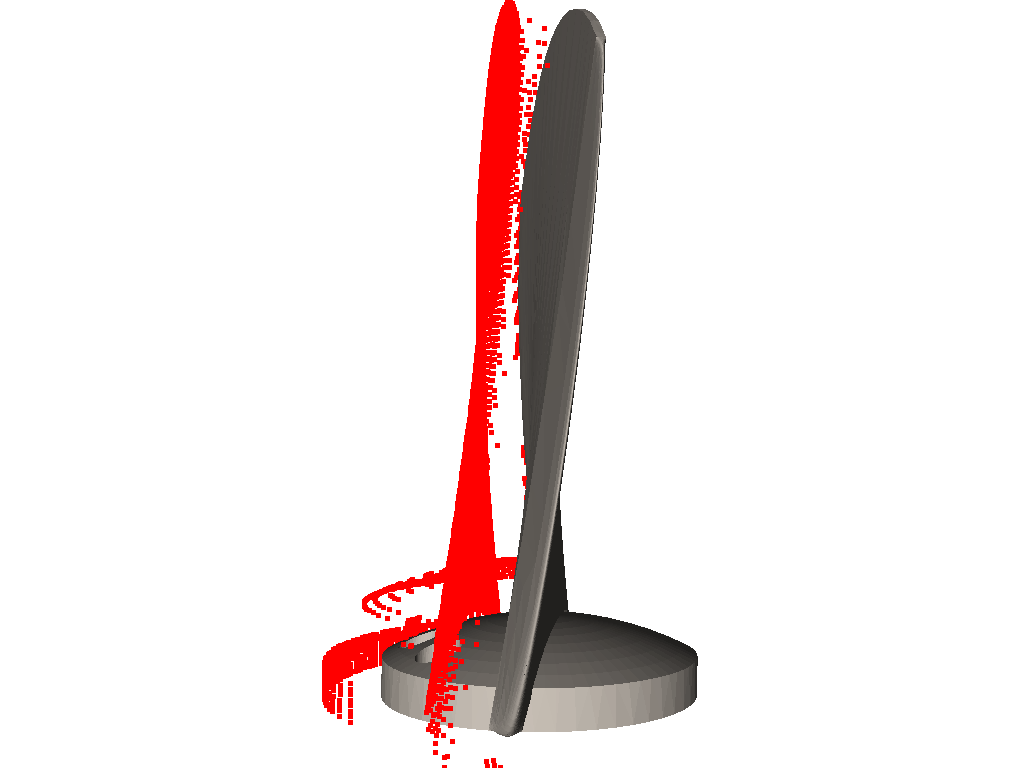
\includegraphics[width=.3\columnwidth]{figs/amostrapa1.png}
	\caption{Pontos amostrados da pá - vista lateral}
	\label{fig::amostrapa1}
\end{figure}

\begin{figure}[!ht]	
	\centering
	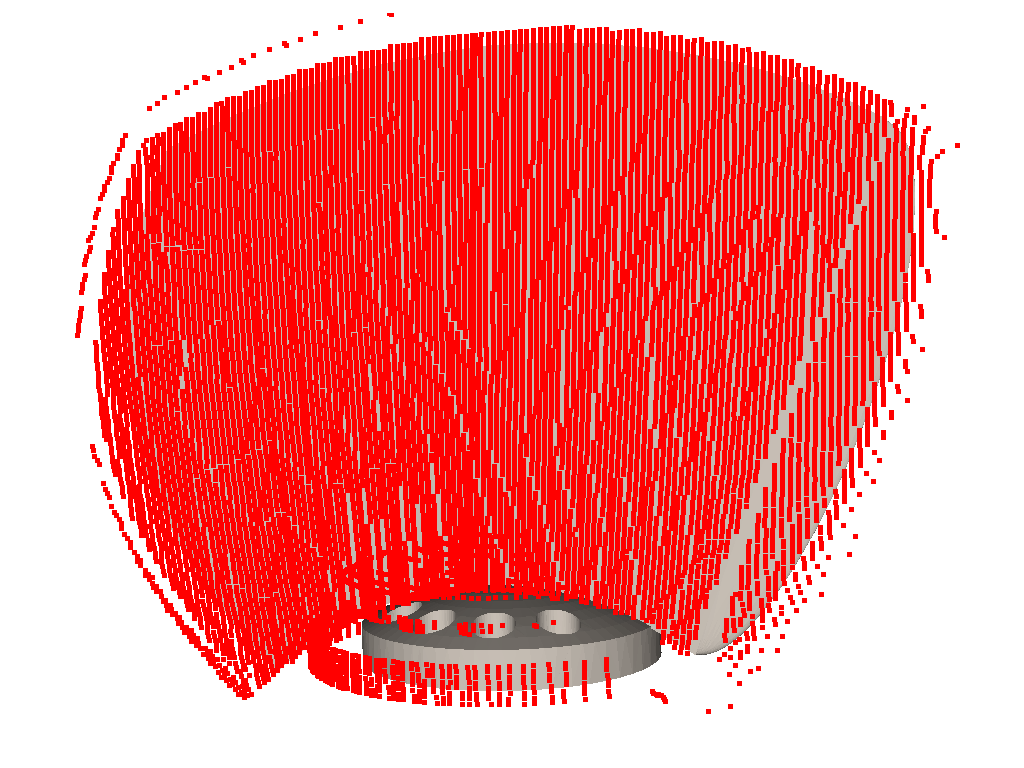
\includegraphics[width=.3\columnwidth]{figs/amostrapa2.png}
	\caption{Pontos amostrados da pá - vista frontal}
	\label{fig::amostrapa2}
\end{figure}

A técnica AABB realizada no OpenRAVE é semelhante ao
planejamento inicial para uma tarefa do tipo \textit{grasping}, na qual um robô
manipulador deve agarrar um objeto e, portanto, necessita reconhecer o seu
formato, e como se aproximar pelos vetores normais. Como a pá da turbina, alguns
objetos podem ser muito irregulares, de forma que amostras uniformes na
superfície do bloco não geram amostras uniformes na superfície do objeto
(figuras~\ref{fig::boundingbox} e ~\ref{fig::sampling}). A fim de garantir um
passo de amostragem próximo à resolução mínima do revestimento (3 mm), é
realizada uma superamostragem de 0.1 mm no bloco e aplica-se um filtro de 1 mm
na superfície da pá. O filtro busca por pontos na pá com distância inferior a 1
mm, mantendo um e deletando os vizinhos próximos. Em relação ao custo
computacional, o filtro foi implementado de maneira ótima pela técnica do
KDTree \cite{wald2006building}.

\begin{figure}[!ht]	
	\centering
	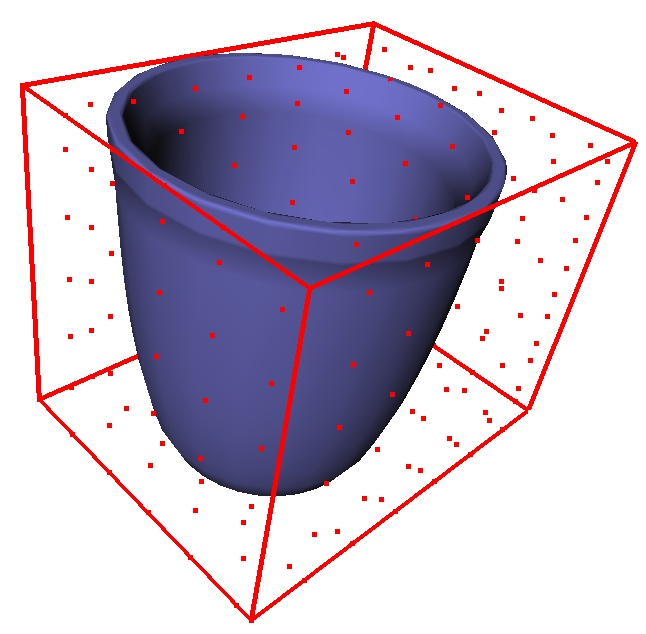
\includegraphics[width=.3\columnwidth]{figs/boundingbox.jpg}
	\caption{Amostras uniformes na superfície do bloco.}
	\label{fig::boundingbox}
\end{figure}

\begin{figure}[!ht]
	\centering	
	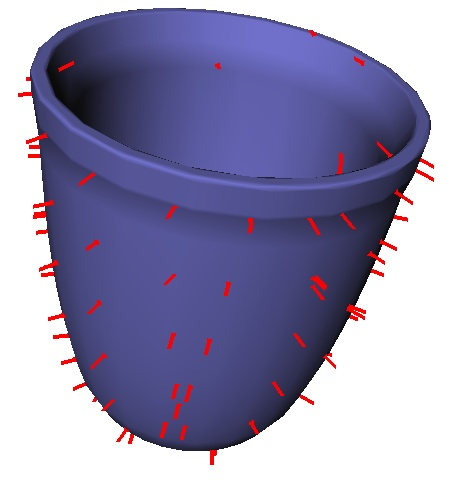
\includegraphics[width=.3\columnwidth]{figs/sampling.jpg}
	\caption{Amostras não uniformes na superfície do objeto.}
	\label{fig::sampling}
\end{figure}